\chapter{Επιταχυντικό Σύστημα}
	Για την ανάλυση του πειράματος STAR στο BNL θα ξεκινήσουμε με το επιταχυντικό σύστημα που δίνει την απαιτούμενη ενέργεια στα σωματίδια, μετά θα ασχοληθούμε με το τι ακριβώς αποτελεί τον ανιχνευτή STAR, ο οποίος είναι ένας από τους τέσσερις ανιχνευτές που κατά περιόδους έχουν ανιχνεύση γεγινότα από τον RHIC και ο μοναδικός εν ενεργεία, και έπειτα θα εξετάσουμε τί είναι αυτό το οποίο παράγεται στην συγκρούσεις και μερικές παραμέτρους για την μελέτη του.
	
	%παράγεται από αυτές τις συγκρούσεις και εν τέλει θα εξετάσουμε τον τρόπο με τον οποίο αυτά τα προϊόντα ανιχνεύονται από  τον ανιχνευτή STAR που είναι ένας από τους τέσσερις ανιχνευτές που κατά περιόδους έχουν ανιχνεύσει γεγονότα από τον RHIC και ο μόνος εν ενεργεία σήμερα. 
	
%\textcolor{red}{Πρωτού αρχίσουμε, ας αναφέρουμε κάποια τεχνικά χαρακτηριστικά του RHIC. Πρόκειται για τον μοναδικό εν ενεργεία επιταχυντή στις Η.Π.Α. και έχει περιφέρεια 3.8 χιλιόμετρα. Η ενέργεια της δέσμης στο σύστημα κέντρου μάζας του είναι}

	Ο RHIC πρόκειται για τον μοναδικό εν ενεργεία επιταχυντή υψηλών ενεργειών στις Η.Π.Α. και για τον μοναδικό επιταχυντή παγκοσμίως που μπορεί να επιταχύνει πολωμένες δέσμες πρωτονίων. Η περιφέρειά του είναι 3.8 χιλιόμετρο και η ενέργειες στο κέντρο μάζας διαφέρουν ανάλογα με τα σωματίδια της δέσμης, ενδεικτικά για τον χρυσό είναι $100GeV/n$.

\begin{figure}[h!]\label{fig2.1}
	\centering
	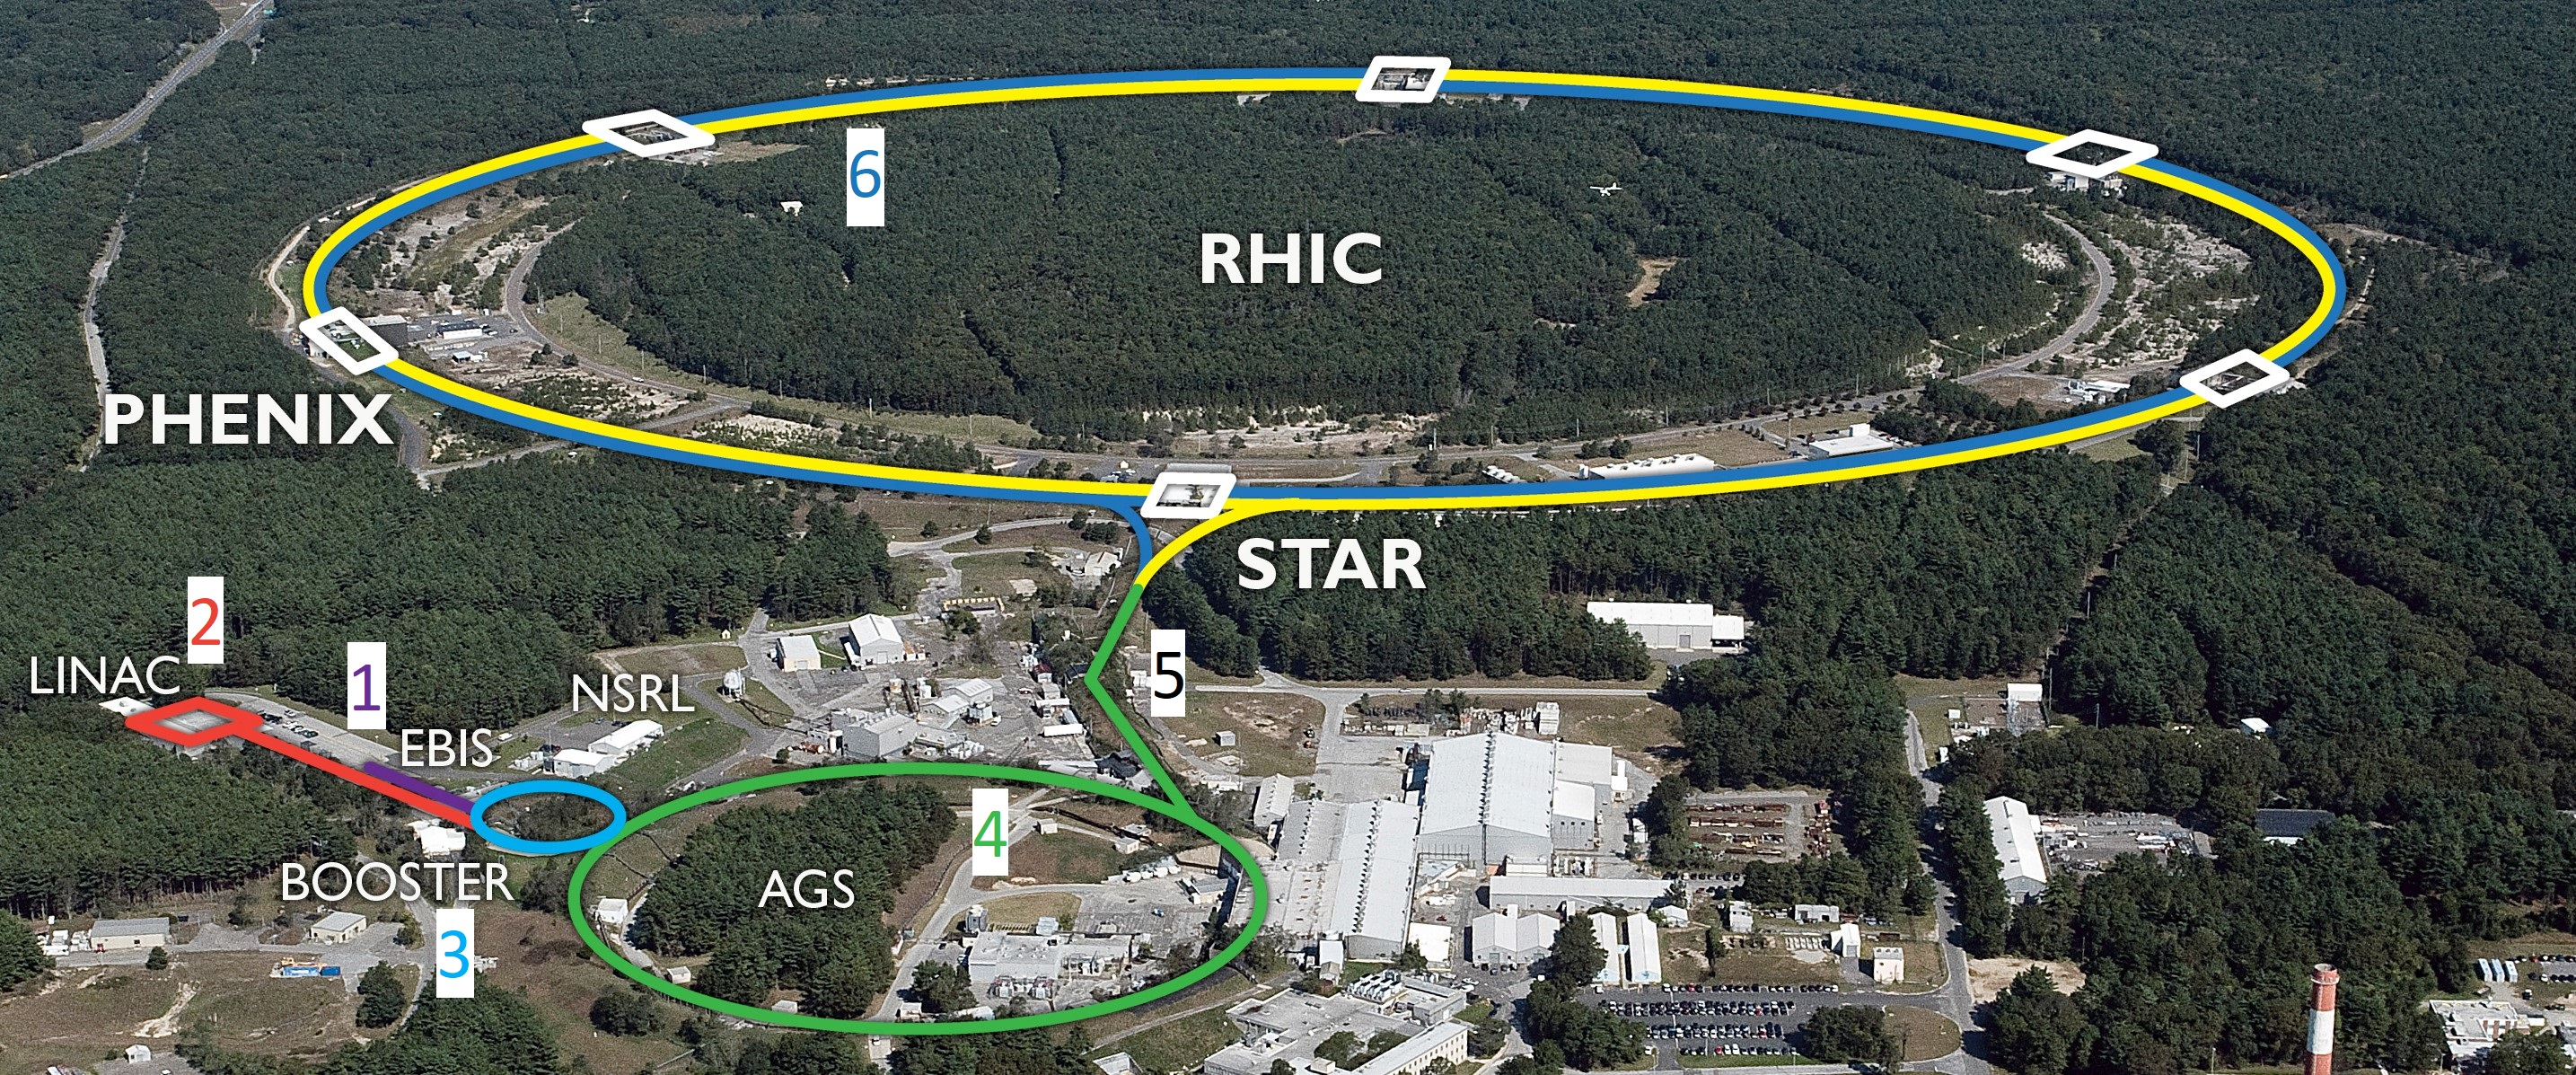
\includegraphics[scale=0.5]{Accelerating_System/written}
	\caption{Εικόνα του επιταχυντικού Συστήμαος στο BNL [1] Electron Beam Ion Source, [2] Linax, [3] Booster Synchrotron, [4] Alternating Gradient Synchrotron, [5] ACS to RHIC Line, [6] RHIC}
\end{figure}

	\section{Η Πορεία των Βαρέων Ιόντων}
	Ένα από τα πειράματα στον RHIC είναι η σύγκρουση δεσμών βαρέων ιόντων, στην αρχή της λειτουργίας του κυρίως Χρυσού, ενώ έπειτα από μία αναβάθμιση του συστήματος δημιουργίας των ιόντων είναι εφικτή και η σύγκρουση βαρύτερων ιόντων όπως Ουρανίου. Μετά την δημιουργία τους, προκειμένου να τους δώσουμε τα επιθυμητά χαρακτηριστικά, τις εισάγουμε διαδοχικά σε τρεις επιταχυντές πρωτού φτάσουν τελικά στον RHIC. Ο κάθε ένας από αυτούς πραγματοποιεί μία διαφορετική επεξεργασία της δέσμης.
	
	\subsection{Electron Beam Ion Source (EBIS)}
	Στις αρχές της λειτουργίας του πειράματος, από το 2000 έως το 2010, η πηγή των ιόντων ήταν ένα σύστημα που λέγεται Tandem Van de Graaff (TVGD). Πρόκειται για δύο διαδοχικούς και ανεξάρτητους επιταχυντές TVGD που μπορούσαν να επιταχύνουν ιόντα προερχόμενα από διαφορετικές πηγές. 
	Ωστόσο, επειδή αυτοί οι επιταχυντές ήταν παλιάς τεχνολογίας έθεταν περιορισμούς ως προς την δυνατότητα δημιουργίας δέσμης από διαφορετικά ιόντα και η αρχή λειτουργίας τους επίτασσε η αρχική πηγή να παρέχει μόνο ανιόντα. Υπήρχαν δύο περιοχές, η πρώτη με διαφορά δυναμικού +V ενώ η δεύτερη με –V. 
	Έτσι αναγκαστικά έπρεπε να ξεκινήσουν με ανιόντα, να τα επιταχύνουν στην πρώτη περιοχή, έπειτα στην μεση των δύο περιοχών να τοποθετήσουν ένα υλικό το οποίο θα απομάκρυνε δύο ηλεκτρόνια έτσι ώστε να δημιουργήσουν τα επιθυμητά κατιόντα τα οποία θα επιταχύνονταν στην δεύτερη περιοχή.
	
	Ήταν λοιπόν αναγκαία η αντικατάσταση του εν λόγω συστήματος για την αρχική δημιουργία και επιτάχυνση των ιόντων  και το 2010 ξεκίνησε την λειτουργία του το σύστημα Electron Beam Ion Source (EBIS). Το EBIS έχει την δυνατότητα να ξεκινάει την λειτουργία του όχι μόνο με ανιόντα, αλλά ακόμη με κατιόντα και ουδέτερα άτομα και επιπλέον μπορεί να εναλλάσσει τις δέσμες που επιταχύνει μέσα σε ένα δευτερόλεπτο. Δηλαδή, αν προετοιμάζει μία δέσμη με κατιόντα χρυσού για τον RHIC, μόλις ένα δευτερόλεπτο μετά μπορεί να προετοιμάσει μία δέσμη από διαφορετικό στοιχείο για άλλες ανάγκες του BNL. 
	
	Τo EBIS απότελείται από έναν θάλαμο 1.5m ο οποίος περικλείεται από έναν κυκλινδρικό υπεραγώγιμο μαγνήτη. Έτσι δημιουργείται στο εσωτερικό του θαλάμου μία μαγνητική παγίδα στην οποία  είναι εγκλωβισμένα τα ιόντα που εισάγονται από εξωτερική πηγή. Στην μία άκρη του θαλάμου υπάρχει ένα Electron Gun που εκπέμπει ηλεκτρόνια 10Α μέσω θερμιονικής εκπομπής, ενώ στην άλλη υπάρχει ένας συλλέκτης ηλεκτρονίων. 
	Καθώς εισάγονται τα ιόντα που θέλουμε να δημιουργήσουμε εισάγονται παγίδα ως αερίο ουδέτερων ατόμων ή ιονισμένων με $1^+$, περνάει από την ίδια περιοχή η δέσμη ηλεκτρονίων. 
	Η δέσμη ιονίζει περεταίρω τα ιόντα τα οποία μπορούν να εξαχθούν οποιαδήποτε στιγμή έχουν αποκτήσει το απαιτούμενο φορτίο. Για την χρήση στον RHIC, χρησιμοποιείται συχνά χρυσός ο οποίος παραμένει στην παγίδα έως ότου γίνει $ Au^{+32}$.% To +32 έχει να κάνει με τις προδιαγραφές των επόμενων προ-επιταχυντών μέσω των οποίων περνά πριν καταλήξει στον RHIC.
	
	Στο τέλος θαλάμου υπάρχει ένας ηλεκτροστατικός φακός ο οποίος χρησιμεύει στην διεύρυνσης της δέσμης κατά την εισαγωγή της στην παγίδα και για την εστίαση κατά την εξαγωγή της. Αφού εξαχθεί, η δέσμη οδηγείται σε δύο αρχικούς γραμμικούς προεπιταχυντές. Ο πρώτος είναι ένας Radio-Frequency Quadrupole (RFQ Linac), ο οποίος είναι ένας κυλινδρικός κυματοδηγός με τέσσερα ηλεκτρόδια τοποθετημένα σε σχήμα σταυρού, όπως φαίνεται στην Εικόνα (\ref{fig2.2}). Στο εσωτερικό του, δεδομένου ότι υπάρχουν συνθήκες κενού, από την κυματική εξίσωση  $\Box^2 \textbf{E}=0$ με συνοριακές συνθήκες $\textbf{E}_\parallel =0 \& \textbf{B}_\perp = 0$ μπορούν να δημιουργηθούν Transverse Electric Modes ($TE_{nlm}$) και Transverse Magnetic Mοdes ($TM_{nlm}$). Επειδή η κοιλότητα έχει τα τέσσερα ηλεκτρόδια, μπορούμε να επιβάλλουμε τον $TE_{210}$ καθώς αυτός είναι βολικός για τον περιορισμό της δέσμης και την διατήρηση της εστίασής της.
	
	Πιο συγκεκριμένα, θεωρούμε πως η δέσμη θετικών ιόντων εισέρχεται στον RFQ με ακριβώς κυκλικό σχήμα, ταχύτητα β και πως το ΗΜ κύμα έχει συχνότητα f. Επειδή οι πολικότητες στα τέσσερα ηλεκτρόδια είναι εναλλάξ, η δέσμη θα συμπιεστεί στην κατεύθυνση των θετικών ηλεκτροδίων ενώ θα αποσυμπιεστεί στην κατεύθυνση των αρνητικών δημιουργώντας μία έλλειψη (Εικόνα \ref{fig2.2}). Έπειτα από μισή περίοδο, οι παραπάνω δυνάμεις αλλάζουν πρόσημο οδηγώντας την σε συμπίεση/αποσυμπίεση κατά τους αντίθετους άξονες. 
	Μέχρι στιγμής δεν έχουμε καταφέρει κάτι ως προς την επιτάχυνση της δέσμης. Το μόνο που συμβαίνει είναι ότι η δέσμη να ταξιδεύει εντός ενός κυματοδηγού, παρουσία Η/Μ πεδίου που προέρχεται από στάσιμα ραδιοκύματα με αποτέλεσμα την εστίασή της εξαιτίας της γεωμετρίας του κυματοδηγού. Τώρα, αν μεταβάλλουμε την απόσταση των απέναντι ηλεκτροδίων με περιοδικό τρόπο ως προς τον χώρο (π.χ. ημιτονοειδώς) , με περίοδο $\beta\lambda/2$, δημιουργούνται και διαμήκεις συνιστώσες ΗΜ πεδίου που επιταχύνουν τα σωματίδια της δέσμης (Εικόνα (\ref{fig2.3})).
	
	
	\begin{figure}[h!]
\centering
\begin{minipage}[c]{0.5\textwidth}
  \centering
  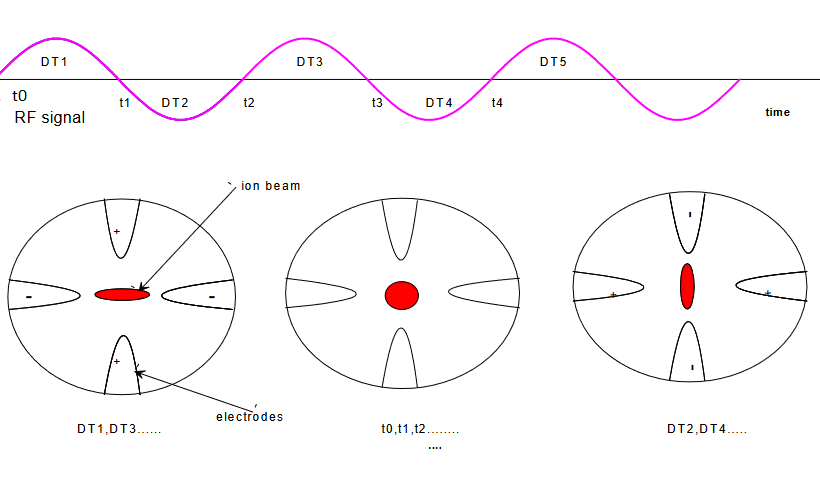
\includegraphics[width=1.1\linewidth]{Accelerating_System/quadtrupole.png}
  \caption{Τομή του κυματοδηγού στον RFQ}
  \label{fig2.2}
\end{minipage}\hfill
\begin{minipage}[r]{0.5\textwidth}\hfill
	\centering
	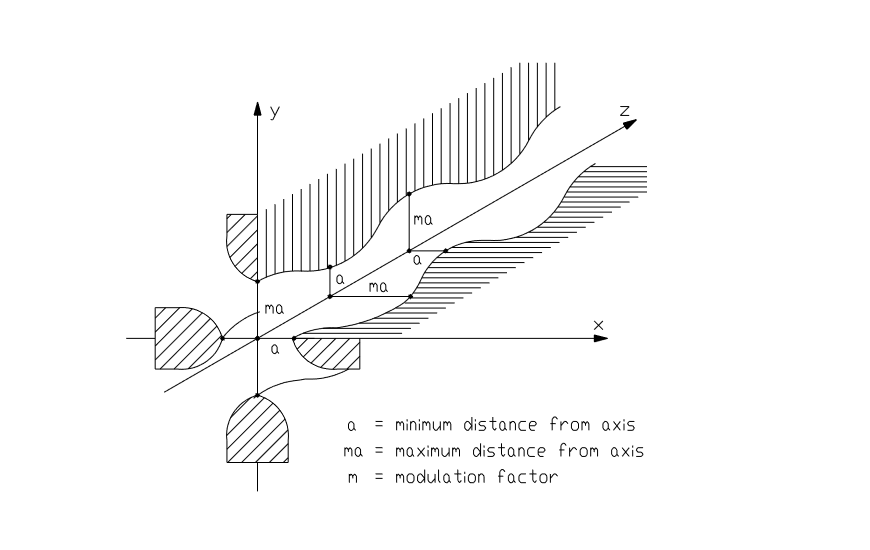
\includegraphics[width=1.3\linewidth]{Accelerating_System/long_modulation_of_wave_guide_in_RFQ.png}
	\caption{Διαμήκης περιοδική μεταβολή του κυματοδηγού για την επιτάχυνση της δέσμης}
	\label{fig2.3}
\end{minipage}
\end{figure}

%	\begin{figure}[!tbp]
%  \centering
%  \subfloat[][Συμπεριφορά του ΤΕ εντός της κοιλότητας]{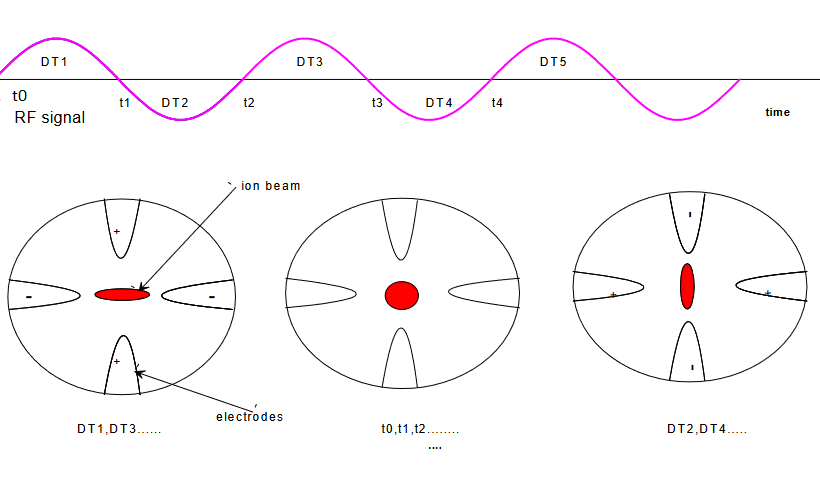
\includegraphics[width=0.5\textwidth]{Accelerating_System/quadtrupole.png}\label{fig:f1}}
%  \hfill
%  \subfloat[][Χωρική μεταβολή του RFQ]{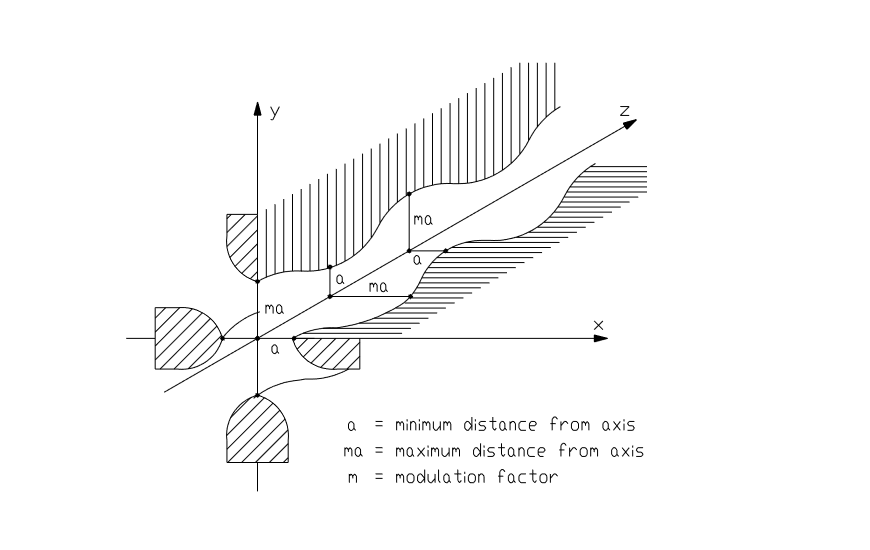
\includegraphics[width=0.5\textwidth]{Accelerating_System/long_modulation_of_wave_guide_in_RFQ.png}\label{fig:f2}}
%  \end{figure}


%\begin{figure}[!h] 
%	\centering 
%	\begin{minipage}[t]{4cm} 
%		\centering 
%		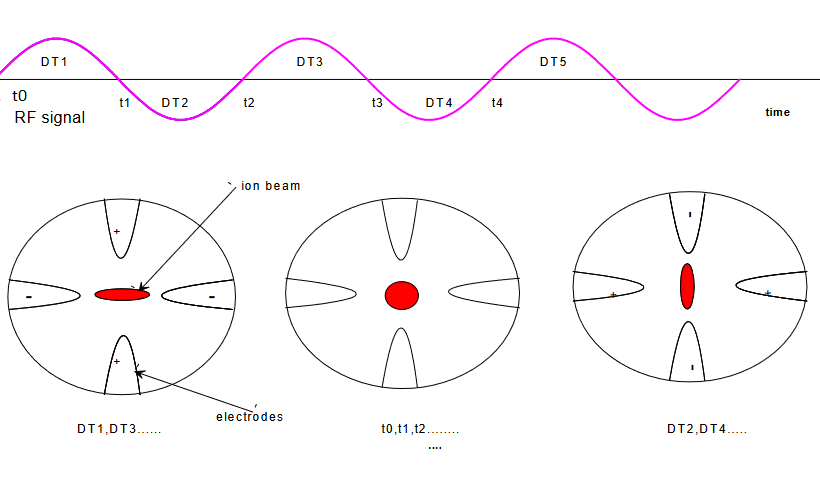
\includegraphics[scale=0.8]{Accelerating_System/quadtrupole.png} 
%		\caption{Caméra thermique 1} 
%	\end{minipage} 
%	\hspace{3cm} 
%	\begin{minipage}[t]{4cm} 
%		\centering 
%		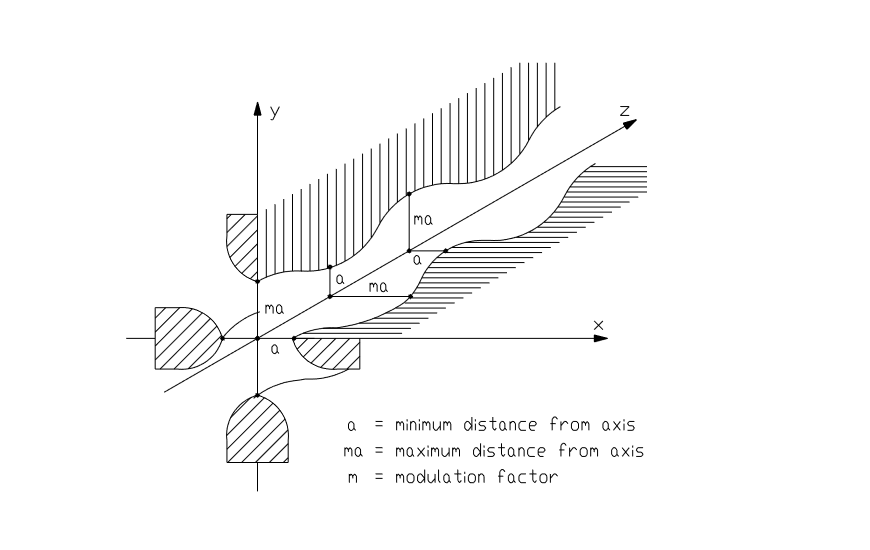
\includegraphics[scale=0.8]{Accelerating_System/long_modulation_of_wave_guide_in_RFQ.png} 
%		\caption{Caméra thermique 2} 
%	\end{minipage} 
%\end{figure} 



	
	Κατά την εξαγωγή της δέσμης από τον RFQ, εισάγεται σε έναν γραμμικό επιταχυντή IH-Linac (Interdigital H-Linear Accelerator). Ο επιταχυντής αποτελείται από μία κοιλότητα στην οποία είναι τοποθετημένοι διακριτοί ομοαξονικοί σωλήνες στο ενδιάμεσο των οποίων υπάρχει κενός χώρος. Ακόμη, σε όλον αυτόν τον χώρο υπάρχει ηλεκτρικό πεδίο που προέρχεται από ραδιοκύματα συχνότητας $f_{RF}$. 
	%Ο επιταχυντής αποτελείται από μία κοιλότητα στην οποία υπάρχει ηλεκτρικό πεδίο που προέρχεται από ραδιοκύματα. 
	
	
	Συνεπώς, η ηλεκτρική συνιστώσα της δύναμης που δέχεται το κάθε σωματίδιο της δέσμης είναι 
	\begin{equation}\label{eq1}
		\bm{F_E} = q \bm{E} = q \bm{E_0}e^{i\omega t}cos(ks),  q>0 
	\end{equation}
	Άρα η ώθηση που κερδίζει δίνεται από την ολοκλήρωση του $2^{ου}$ νόμου του Newton
	\begin{align*}\label{eq2}
		\odv{mc\gamma\bm{\beta}}{t} = q \bm{E} \Rightarrow \\
		\Delta p = m(\gamma\bm{\beta}-\gamma_0\bm{\beta_0}) = q \int\bm{E}dt \numberthis
	\end{align*}
	
	Συνεπώς όταν το ηλεκτρικό πεδίο παίρνει αρνητικές τιμές, η ώθηση θα είναι αρνητική και τα σωματίδια θα χάνουν ορμή. Για αν αποφύγουμε το παραπάνω πρόβλημα μπορούμε να τοποθετήσουμε στο εσωτερικό της κοιλότητας ομοαξονικούς σωλήνες μεταξύ των οποίων θα υπάρχει κενός χώρος. Οι σωλήνες θα είναι έτσι τοποθετημένοι ώστε όταν το πεδίο, άρα η ώθηση γίνεται αρνητική τα σωματίδια να περνάνε από το εσωτερικό του. 
	Τότε, αυτοί θα δρουν ως κλωβοί Faraday και θα θωρακίζουν την δέσμη από το πεδίο στο εξωτερικό τους το οποίο θα την επιβράδυνε. Ταυτόχρονα δεν αλλοιώνουν σημαντικά τους κάθετους ρυθμούς του πεδίου στον ενδιάμεσο χώρο. 
	Επομένως, εμείς θέλουμε τα σωματίδιά μας να εισέλθουν στον χώρο εκτός των σωλήνων όταν το πεδίο θα γίνεται επιταχυντικό, δηλαδή για διάστημα $\Delta t_{RF}=1/2f_{RF}$   σε κάθε περίοδο. Για να έχουμε την βέλτιστη επιτάχυνση, θα πρέπει η αλληλεπίδραση σωματιδίου-κύματος να ξεκινάει για ίδια φάση του κύματος. 
	Έτσι η επιτάχυνση κάθε περιοχή θα είναι ίδια και στο πέρας της j-οστής περιοχής θα είναι απλώς $j\cdot\alpha_1$.  Αυτή η φάση που πρέπει να έχει το κύμα καλείται synchronous phase και συμβολίζεται $\psi_s$. Άρα θα πρέπει να ισχύουν: 
	\begin{align*}\label{eq3}
		\psi_s         =& \omega t_j - kz_j   = const.\Rightarrow\\
		\odv{\psi_s}{t}=& \omega - k\beta_jc  = 0 \numberthis
	\end{align*}
	
	Ο χρόνος που μένουν τα σωματίδια εντός και εκτός των επιταχυντικών περιοχών είναι μισή περίοδος, άρα η διαφορά φάσης που βλέπουν στις δύο περιοχές εισόδου-εξόδου είναι $\pi$.
	
  Δεν θα πρέπει να αμελήσουμε το γεγονός ότι η απόσταση που διανύει η δέσμη σε αυτόν τον χρόνο αυξάνεται καθώς αυτή κινείται εντός του επιταχυντή. Όταν έχει περάσει από την j-οστή περιοχή επιτάχυνσης θα έχει ταχύτητα $u_i$ και η απόσταση που θα διανύει σε $1/2f_{RF}$ είναι 
	\begin{align}\label{eq4}
		l_i = \frac{u_i}{2f_{RF}} = \frac{u_i\lambda_{RF}}{2c} = \frac{\beta_i\lambda_{RF}}{2}
	\end{align}
	
	Η ενέργεια που κερδίζει με κάθε διέλευση από την j-oστή περιοχή επιτάχυνσης μήκους $l_j$ είναι
		\begin{align}\label{eq5}
			\Delta E_{kin} =q \int_{r_j}^{r_{j+1}}\bm{E}\cdot d\bm{s} = q E_{0s}e^{i(\omega t_j+\pi)} \left(-\frac{sink_jl_j}{k_j}-0\right) = \frac{qE_{0s}e^{i\omega t_j}sink_jl_j}{k_j}
		\end{align}
		
		Άρα αν θεωρήσουμε ως $T_0$ την κινητική ενέργεια με την οποία εισέρχεται στον IH-Linac, από την συνολική κινητική ενέργεια στην j επιταχυντική περιοχή και στο μη σχετικιστικό όριο προκύπτει και η ταχύτητα που θα έχει η δέσμη 
			\begin{align*}\label{eq6}
					T_j       =& T_0 + j\Delta E_{kin} = m(\gamma -1)c^2 \xRightarrow{non relat. limit} \\ 
					\beta_j^2 =& \frac{u_j^2}{c^2} = \frac{2(T_0 +j\Delta E_{kin})}{mc^2}  \numberthis
			\end{align*}
			
			Συνεπώς από τις σχέσεις (\ref{eq3}), (\ref{eq6}) έχουμε ότι το μήκος των σωλήνων θα αυξάνεται $\sim\sqrt{j}$. Ακόμη, δεν θα πρέπει να χρησιομποιήσουμε $\psi_s=\pi/2$ που αντιστοιχεί στο μέγιστο του πεδίου άρα στο μέγιστο της δύναμης που δέχονται τα σωματίδια. 
			Αυτό διότι όταν έχουμε μεγάλο αριθμό j σταδίων επιτάχυνσης τότε η ταχύτητα των σωματιδίων θα αποκλίνει από την θεωρητικά σχεδιασμένη, επομένως τα σωματίδια θα βλέπουν διαφορετική φάση του κύματος καθώς εισέρχονται στην περιοχή επιτάχυνσης και ο συγχρονισμός κύματος-σωματιδίου θα χάνεται. 
			Ωστόσο αν χρησιμοποιήσουμε $\psi_s<\pi/2$, τότε παρ'ολο που δεν έχουμε την μέγιστη επιτάχυνση, αν η ταχύτητα αρχίσει να αποκλίνει έπειτα από κάποια στάδια, τα σωματίδια θα βλέπουν το κύμα σε διαφορετική φάση $\psi_s\pm\Delta\psi$, ανάλογα με το αν έχουν επιταχυνθεί περισσότερο ή λιγότερο από το αναμενόμενο. Έτσι, αν για παράδειγμα κάποιο έχει μεγαλύτερη ταχύτητα από την αναμενόμενη, θα βλέπει το κύμα σε μικρότερη φάση $\psi_s-\Delta\psi$, άρα σε μικρότερη τιμή του πεδίου του με αποτέλεσμα να επιταχύνεται λιγότερο από όσα έχουν επιταχυνθεί λιγότερο από το επιθυμητό. Όσα έχουν επιταχυνθεί λιγότερο, θα βλέπουν το κύμα σε μεγαλύτερη φάση, άρα μεγαλύτερο πεδίο.
			
			
			Κατ’ αυτόν τον τρόπο, επιτυγχάνεται ένα κλείδωμα φάσης που οδηγεί σε σχεδόν ομοιόμορφη επιτάχυνση όλων των σωματιδίων της δέσμης. Φυσικά, οι εξισώσεις και οι υπολογισμοί σε έναν πραγματικό HI-Linac είναι πιο πολύπλοκες από τις παραπάνω καθώς θα πρέπει να λάβουμε υπ΄όψιν και άλλες παραμέτρους.%
%			, όπως η αλλοίωση του πεδίου από την τοποθέτηση των σωλήνων.
			 Ένα σχήμα HI-Linac φαίνεται στην Εικόνα (\ref{fig2.4}).
			
			\begin{figure}[h!]
				\centering
				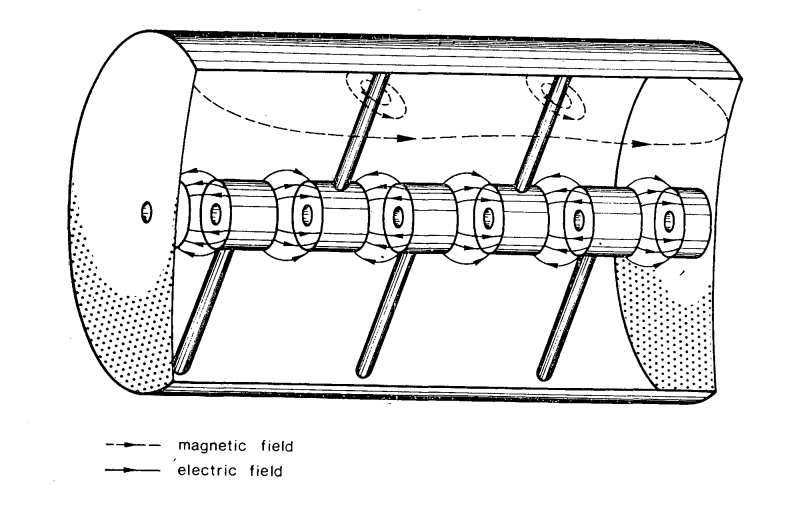
\includegraphics[scale=0.5]{linac.png}
				\caption{Σχέδιο HI-Linac}
				\label{fig2.4}
			\end{figure}
			
			
			
			
			
			
			
			